\documentclass[twoside]{book}

% Packages required by doxygen
\usepackage{fixltx2e}
\usepackage{calc}
\usepackage{doxygen}
\usepackage[export]{adjustbox} % also loads graphicx
\usepackage{graphicx}
\usepackage[utf8]{inputenc}
\usepackage{makeidx}
\usepackage{multicol}
\usepackage{multirow}
\PassOptionsToPackage{warn}{textcomp}
\usepackage{textcomp}
\usepackage[nointegrals]{wasysym}
\usepackage[table]{xcolor}

% Font selection
\usepackage[T1]{fontenc}
\usepackage[scaled=.90]{helvet}
\usepackage{courier}
\usepackage{amssymb}
\usepackage{sectsty}
\renewcommand{\familydefault}{\sfdefault}
\allsectionsfont{%
  \fontseries{bc}\selectfont%
  \color{darkgray}%
}
\renewcommand{\DoxyLabelFont}{%
  \fontseries{bc}\selectfont%
  \color{darkgray}%
}
\newcommand{\+}{\discretionary{\mbox{\scriptsize$\hookleftarrow$}}{}{}}

% Page & text layout
\usepackage{geometry}
\geometry{%
  a4paper,%
  top=2.5cm,%
  bottom=2.5cm,%
  left=2.5cm,%
  right=2.5cm%
}
\tolerance=750
\hfuzz=15pt
\hbadness=750
\setlength{\emergencystretch}{15pt}
\setlength{\parindent}{0cm}
\setlength{\parskip}{3ex plus 2ex minus 2ex}
\makeatletter
\renewcommand{\paragraph}{%
  \@startsection{paragraph}{4}{0ex}{-1.0ex}{1.0ex}{%
    \normalfont\normalsize\bfseries\SS@parafont%
  }%
}
\renewcommand{\subparagraph}{%
  \@startsection{subparagraph}{5}{0ex}{-1.0ex}{1.0ex}{%
    \normalfont\normalsize\bfseries\SS@subparafont%
  }%
}
\makeatother

% Headers & footers
\usepackage{fancyhdr}
\pagestyle{fancyplain}
\fancyhead[LE]{\fancyplain{}{\bfseries\thepage}}
\fancyhead[CE]{\fancyplain{}{}}
\fancyhead[RE]{\fancyplain{}{\bfseries\leftmark}}
\fancyhead[LO]{\fancyplain{}{\bfseries\rightmark}}
\fancyhead[CO]{\fancyplain{}{}}
\fancyhead[RO]{\fancyplain{}{\bfseries\thepage}}
\fancyfoot[LE]{\fancyplain{}{}}
\fancyfoot[CE]{\fancyplain{}{}}
\fancyfoot[RE]{\fancyplain{}{\bfseries\scriptsize Generated by Doxygen }}
\fancyfoot[LO]{\fancyplain{}{\bfseries\scriptsize Generated by Doxygen }}
\fancyfoot[CO]{\fancyplain{}{}}
\fancyfoot[RO]{\fancyplain{}{}}
\renewcommand{\footrulewidth}{0.4pt}
\renewcommand{\chaptermark}[1]{%
  \markboth{#1}{}%
}
\renewcommand{\sectionmark}[1]{%
  \markright{\thesection\ #1}%
}

% Indices & bibliography
\usepackage{natbib}
\usepackage[titles]{tocloft}
\setcounter{tocdepth}{3}
\setcounter{secnumdepth}{5}
\makeindex

% Hyperlinks (required, but should be loaded last)
\usepackage{ifpdf}
\ifpdf
  \usepackage[pdftex,pagebackref=true]{hyperref}
\else
  \usepackage[ps2pdf,pagebackref=true]{hyperref}
\fi
\hypersetup{%
  colorlinks=true,%
  linkcolor=blue,%
  citecolor=blue,%
  unicode%
}

% Custom commands
\newcommand{\clearemptydoublepage}{%
  \newpage{\pagestyle{empty}\cleardoublepage}%
}

\usepackage{caption}
\captionsetup{labelsep=space,justification=centering,font={bf},singlelinecheck=off,skip=4pt,position=top}

%===== C O N T E N T S =====

\begin{document}

% Titlepage & ToC
\hypersetup{pageanchor=false,
             bookmarksnumbered=true,
             pdfencoding=unicode
            }
\pagenumbering{alph}
\begin{titlepage}
\vspace*{7cm}
\begin{center}%
{\Large Audio\+Engine }\\
\vspace*{1cm}
{\large Generated by Doxygen 1.8.13}\\
\end{center}
\end{titlepage}
\clearemptydoublepage
\pagenumbering{roman}
\tableofcontents
\clearemptydoublepage
\pagenumbering{arabic}
\hypersetup{pageanchor=true}

%--- Begin generated contents ---
\chapter{Module Index}
\section{Modules}
Here is a list of all modules\+:\begin{DoxyCompactList}
\item \contentsline{section}{Audio\+Effect}{\pageref{group___audio_effect}}{}
\end{DoxyCompactList}

\chapter{Hierarchical Index}
\section{Class Hierarchy}
This inheritance list is sorted roughly, but not completely, alphabetically\+:\begin{DoxyCompactList}
\item \contentsline{section}{Audio}{\pageref{class_audio}}{}
\item \contentsline{section}{Audio\+Effect}{\pageref{class_audio_effect}}{}
\begin{DoxyCompactList}
\item \contentsline{section}{Fade\+In\+Effect}{\pageref{class_fade_in_effect}}{}
\end{DoxyCompactList}
\item \contentsline{section}{Audio\+Engine}{\pageref{class_audio_engine}}{}
\item \contentsline{section}{Audio\+Storage\+Buffer}{\pageref{class_audio_storage_buffer}}{}
\item \contentsline{section}{Audio\+Time}{\pageref{class_audio_time}}{}
\end{DoxyCompactList}

\chapter{Class Index}
\section{Data Structures}
Here are the data structures with brief descriptions\+:\begin{DoxyCompactList}
\item\contentsline{section}{\hyperlink{struct_audio}{Audio} }{\pageref{struct_audio}}{}
\item\contentsline{section}{\hyperlink{struct_audio_effect}{Audio\+Effect} }{\pageref{struct_audio_effect}}{}
\item\contentsline{section}{\hyperlink{struct_r_i_f_f___h_e_a_d_e_r}{R\+I\+F\+F\+\_\+\+H\+E\+A\+D\+ER} }{\pageref{struct_r_i_f_f___h_e_a_d_e_r}}{}
\item\contentsline{section}{\hyperlink{struct_w_a_v_e___d_a_t_a}{W\+A\+V\+E\+\_\+\+D\+A\+TA} }{\pageref{struct_w_a_v_e___d_a_t_a}}{}
\item\contentsline{section}{\hyperlink{struct_w_a_v_e___h_e_a_d_e_r}{W\+A\+V\+E\+\_\+\+H\+E\+A\+D\+ER} }{\pageref{struct_w_a_v_e___h_e_a_d_e_r}}{}
\end{DoxyCompactList}

\chapter{Module Documentation}
\hypertarget{group___audio_effect}{}\section{Audio\+Effect}
\label{group___audio_effect}\index{Audio\+Effect@{Audio\+Effect}}


Base class for Audio\+Effects.  


\subsection*{Classes}
\begin{DoxyCompactItemize}
\item 
class \hyperlink{class_fade_in_effect}{Fade\+In\+Effect}
\begin{DoxyCompactList}\small\item\em \hyperlink{class_audio}{Audio} effect that applies a fade out effect to audio. \end{DoxyCompactList}\end{DoxyCompactItemize}


\subsection{Detailed Description}
Base class for Audio\+Effects. 

\begin{DoxyWarning}{Warning}
Creating a subclass requires knowledge of working with raw data. 
\end{DoxyWarning}

\chapter{Class Documentation}
\hypertarget{class_audio}{}\section{Audio Class Reference}
\label{class_audio}\index{Audio@{Audio}}


\hyperlink{class_audio}{Audio} class that holds music information. Automatically removes all effects that is still held.  




{\ttfamily \#include $<$Audio.\+h$>$}

\subsection*{Public Member Functions}
\begin{DoxyCompactItemize}
\item 
bool \hyperlink{class_audio_a1014b0af8df3f0eb3dc1e99e86ad43db}{Add\+Effect} (\hyperlink{class_audio_effect}{Audio\+Effect} $\ast$effect)
\begin{DoxyCompactList}\small\item\em Adds an audio effect. \end{DoxyCompactList}\item 
{\footnotesize template$<$typename T $>$ }\\\hyperlink{class_audio_effect}{Audio\+Effect} $\ast$ \hyperlink{class_audio_a63e37ba7c615699db84188fac87dedc9}{Remove\+Effect} ()
\begin{DoxyCompactList}\small\item\em Removes an audio effect. \end{DoxyCompactList}\end{DoxyCompactItemize}
\subsection*{Friends}
\begin{DoxyCompactItemize}
\item 
\mbox{\Hypertarget{class_audio_a234a96133b0b1dbaf4181626861f7c4a}\label{class_audio_a234a96133b0b1dbaf4181626861f7c4a}} 
class {\bfseries Audio\+Engine}
\item 
\mbox{\Hypertarget{class_audio_a7e74df8564d626641971702bfa4a0d5e}\label{class_audio_a7e74df8564d626641971702bfa4a0d5e}} 
class {\bfseries Audio\+Effect}
\end{DoxyCompactItemize}


\subsection{Detailed Description}
\hyperlink{class_audio}{Audio} class that holds music information. Automatically removes all effects that is still held. 


\begin{DoxyParams}{Parameters}
{\em You} & may only obtain an instance of this class through the \hyperlink{class_audio_engine_a7ccb8d2fe6be78b16f457589962aedfe}{Audio\+Engine\+::\+Load()} method. \\
\hline
\end{DoxyParams}


\subsection{Member Function Documentation}
\mbox{\Hypertarget{class_audio_a1014b0af8df3f0eb3dc1e99e86ad43db}\label{class_audio_a1014b0af8df3f0eb3dc1e99e86ad43db}} 
\index{Audio@{Audio}!Add\+Effect@{Add\+Effect}}
\index{Add\+Effect@{Add\+Effect}!Audio@{Audio}}
\subsubsection{\texorpdfstring{Add\+Effect()}{AddEffect()}}
{\footnotesize\ttfamily bool Audio\+::\+Add\+Effect (\begin{DoxyParamCaption}\item[{\hyperlink{class_audio_effect}{Audio\+Effect} $\ast$}]{effect }\end{DoxyParamCaption})}



Adds an audio effect. 


\begin{DoxyParams}{Parameters}
{\em effect} & The audio effect to add. \\
\hline
\end{DoxyParams}
\begin{DoxyReturn}{Returns}
Whether the effect already exists 
\end{DoxyReturn}
\mbox{\Hypertarget{class_audio_a63e37ba7c615699db84188fac87dedc9}\label{class_audio_a63e37ba7c615699db84188fac87dedc9}} 
\index{Audio@{Audio}!Remove\+Effect@{Remove\+Effect}}
\index{Remove\+Effect@{Remove\+Effect}!Audio@{Audio}}
\subsubsection{\texorpdfstring{Remove\+Effect()}{RemoveEffect()}}
{\footnotesize\ttfamily template$<$typename T $>$ \\
\hyperlink{class_audio_effect}{Audio\+Effect} $\ast$ Audio\+::\+Remove\+Effect (\begin{DoxyParamCaption}{ }\end{DoxyParamCaption})}



Removes an audio effect. 


\begin{DoxyTemplParams}{Template Parameters}
{\em T} & The \hyperlink{class_audio_effect}{Audio\+Effect} type to remove. \\
\hline
\end{DoxyTemplParams}
\begin{DoxyReturn}{Returns}
The specified \hyperlink{class_audio_effect}{Audio\+Effect}. 
\end{DoxyReturn}


The documentation for this class was generated from the following files\+:\begin{DoxyCompactItemize}
\item 
C\+:/\+Users/wsheng/\+Documents/\+Neumont/\+Q9/capstone/repo/project/\+Dynamic\+Music/Audio.\+h\item 
C\+:/\+Users/wsheng/\+Documents/\+Neumont/\+Q9/capstone/repo/project/\+Dynamic\+Music/Audio.\+cpp\end{DoxyCompactItemize}

\hypertarget{class_audio_effect}{}\section{Audio\+Effect Class Reference}
\label{class_audio_effect}\index{Audio\+Effect@{Audio\+Effect}}
Inheritance diagram for Audio\+Effect\+:\begin{figure}[H]
\begin{center}
\leavevmode
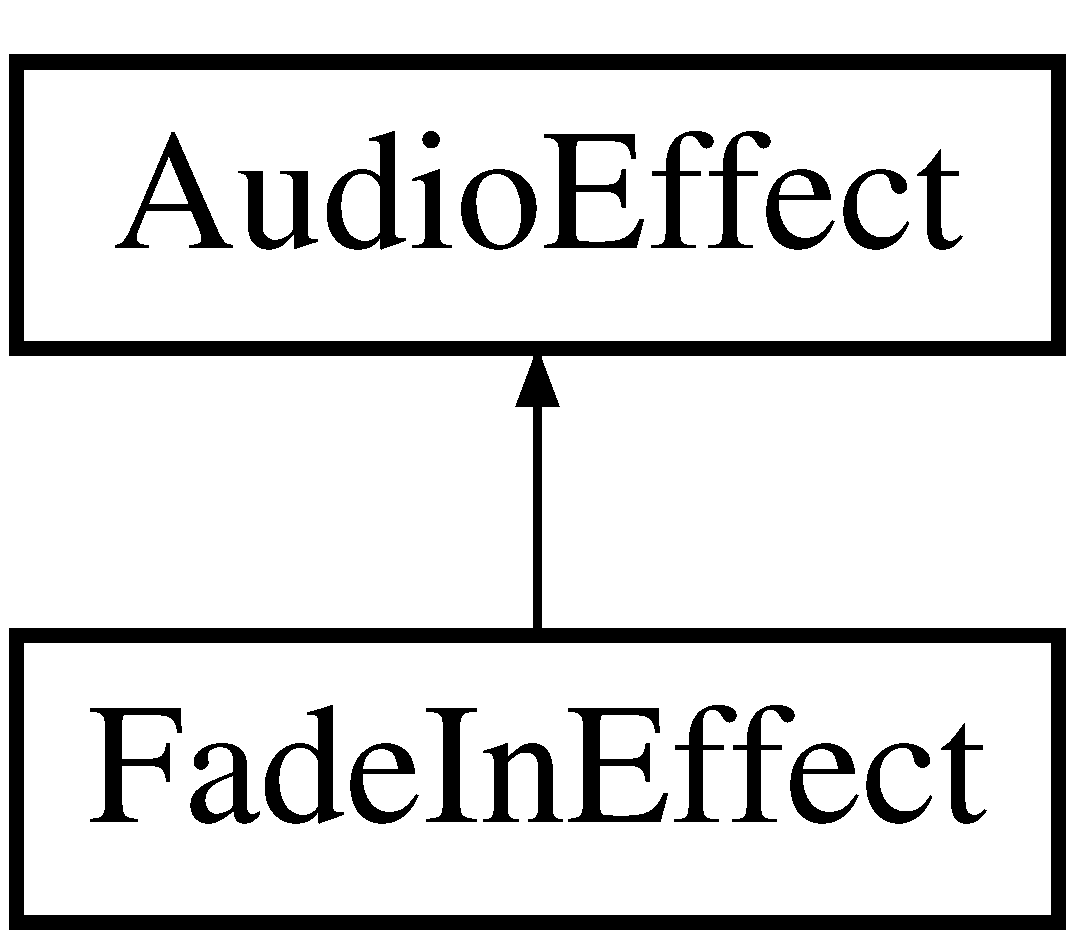
\includegraphics[height=2.000000cm]{class_audio_effect}
\end{center}
\end{figure}
\subsection*{Protected Member Functions}
\begin{DoxyCompactItemize}
\item 
virtual short $\ast$ \hyperlink{class_audio_effect_aa3ef3fe6eb855581fff9db8b69de37cf}{Pre\+Process} (short $\ast$data, int size, unsigned long shorts\+Per\+Second)
\begin{DoxyCompactList}\small\item\em Preprocesses the passed audio data. \end{DoxyCompactList}\item 
virtual short $\ast$ \hyperlink{class_audio_effect_a2b6c7b17eddb589170c977f2d6dc0ec6}{Start\+Process} (short $\ast$data, int size, unsigned long shorts\+Per\+Second)
\begin{DoxyCompactList}\small\item\em Processes the passed audio data. \end{DoxyCompactList}\item 
virtual short $\ast$ \hyperlink{class_audio_effect_aa281bd543b2841eeab97e7f23bed8889}{End\+Process} (short $\ast$data, int size, unsigned long shorts\+Per\+Second)
\begin{DoxyCompactList}\small\item\em Processes the passed audio data. \end{DoxyCompactList}\end{DoxyCompactItemize}
\subsection*{Static Protected Member Functions}
\begin{DoxyCompactItemize}
\item 
static short \hyperlink{class_audio_effect_a206794f66b9e0ca2cde69e970f3f398d}{Clamp} (short in)
\begin{DoxyCompactList}\small\item\em Clamps the passed short to be within audio range. \end{DoxyCompactList}\end{DoxyCompactItemize}
\subsection*{Friends}
\begin{DoxyCompactItemize}
\item 
\mbox{\Hypertarget{class_audio_effect_a234a96133b0b1dbaf4181626861f7c4a}\label{class_audio_effect_a234a96133b0b1dbaf4181626861f7c4a}} 
class {\bfseries Audio\+Engine}
\end{DoxyCompactItemize}


\subsection{Member Function Documentation}
\mbox{\Hypertarget{class_audio_effect_a206794f66b9e0ca2cde69e970f3f398d}\label{class_audio_effect_a206794f66b9e0ca2cde69e970f3f398d}} 
\index{Audio\+Effect@{Audio\+Effect}!Clamp@{Clamp}}
\index{Clamp@{Clamp}!Audio\+Effect@{Audio\+Effect}}
\subsubsection{\texorpdfstring{Clamp()}{Clamp()}}
{\footnotesize\ttfamily static short Audio\+Effect\+::\+Clamp (\begin{DoxyParamCaption}\item[{short}]{in }\end{DoxyParamCaption})\hspace{0.3cm}{\ttfamily [inline]}, {\ttfamily [static]}, {\ttfamily [protected]}}



Clamps the passed short to be within audio range. 


\begin{DoxyParams}{Parameters}
{\em in} & The short \\
\hline
\end{DoxyParams}
\begin{DoxyReturn}{Returns}
The clamped short, within the range -\/0x7fff and 0x7fff 
\end{DoxyReturn}
\mbox{\Hypertarget{class_audio_effect_aa281bd543b2841eeab97e7f23bed8889}\label{class_audio_effect_aa281bd543b2841eeab97e7f23bed8889}} 
\index{Audio\+Effect@{Audio\+Effect}!End\+Process@{End\+Process}}
\index{End\+Process@{End\+Process}!Audio\+Effect@{Audio\+Effect}}
\subsubsection{\texorpdfstring{End\+Process()}{EndProcess()}}
{\footnotesize\ttfamily virtual short$\ast$ Audio\+Effect\+::\+End\+Process (\begin{DoxyParamCaption}\item[{short $\ast$}]{data,  }\item[{int}]{size,  }\item[{unsigned long}]{shorts\+Per\+Second }\end{DoxyParamCaption})\hspace{0.3cm}{\ttfamily [inline]}, {\ttfamily [protected]}, {\ttfamily [virtual]}}



Processes the passed audio data. 

Called by \hyperlink{class_audio_engine_abc49a7e983821493bf5becc5ab25c6a0}{Audio\+Engine\+::\+Swap()}. 
\begin{DoxyParams}{Parameters}
{\em data} & The raw audio data, starting from current song position \\
\hline
{\em size} & The size of the data \\
\hline
{\em shorts\+Per\+Second} & Number of shorts per second (equivalent to bytes per second / 2) \\
\hline
\end{DoxyParams}
\mbox{\Hypertarget{class_audio_effect_aa3ef3fe6eb855581fff9db8b69de37cf}\label{class_audio_effect_aa3ef3fe6eb855581fff9db8b69de37cf}} 
\index{Audio\+Effect@{Audio\+Effect}!Pre\+Process@{Pre\+Process}}
\index{Pre\+Process@{Pre\+Process}!Audio\+Effect@{Audio\+Effect}}
\subsubsection{\texorpdfstring{Pre\+Process()}{PreProcess()}}
{\footnotesize\ttfamily virtual short$\ast$ Audio\+Effect\+::\+Pre\+Process (\begin{DoxyParamCaption}\item[{short $\ast$}]{data,  }\item[{int}]{size,  }\item[{unsigned long}]{shorts\+Per\+Second }\end{DoxyParamCaption})\hspace{0.3cm}{\ttfamily [inline]}, {\ttfamily [protected]}, {\ttfamily [virtual]}}



Preprocesses the passed audio data. 

Called by \hyperlink{class_audio_engine_af4471a467aa56bcad3db5a8a9ce8d733}{Audio\+Engine\+::\+Play()}. This method will only be called once by the \hyperlink{class_audio_engine}{Audio\+Engine}. 
\begin{DoxyParams}{Parameters}
{\em data} & The entire raw audio data \\
\hline
{\em size} & The size of the data \\
\hline
{\em shorts\+Per\+Second} & Number of shorts per second (equivalent to bytes per second / 2) \\
\hline
\end{DoxyParams}
\mbox{\Hypertarget{class_audio_effect_a2b6c7b17eddb589170c977f2d6dc0ec6}\label{class_audio_effect_a2b6c7b17eddb589170c977f2d6dc0ec6}} 
\index{Audio\+Effect@{Audio\+Effect}!Start\+Process@{Start\+Process}}
\index{Start\+Process@{Start\+Process}!Audio\+Effect@{Audio\+Effect}}
\subsubsection{\texorpdfstring{Start\+Process()}{StartProcess()}}
{\footnotesize\ttfamily virtual short$\ast$ Audio\+Effect\+::\+Start\+Process (\begin{DoxyParamCaption}\item[{short $\ast$}]{data,  }\item[{int}]{size,  }\item[{unsigned long}]{shorts\+Per\+Second }\end{DoxyParamCaption})\hspace{0.3cm}{\ttfamily [inline]}, {\ttfamily [protected]}, {\ttfamily [virtual]}}



Processes the passed audio data. 

Called by \hyperlink{class_audio_engine_af4471a467aa56bcad3db5a8a9ce8d733}{Audio\+Engine\+::\+Play()} and \hyperlink{class_audio_engine_abc49a7e983821493bf5becc5ab25c6a0}{Audio\+Engine\+::\+Swap()}. Used when the \hyperlink{class_audio_engine}{Audio\+Engine} plays a song, starting from a specific position. 
\begin{DoxyParams}{Parameters}
{\em data} & The raw audio data, starting from the current song position \\
\hline
{\em size} & The size of the data \\
\hline
{\em shorts\+Per\+Second} & Number of shorts per second (equivalent to bytes per second / 2) \\
\hline
\end{DoxyParams}


The documentation for this class was generated from the following file\+:\begin{DoxyCompactItemize}
\item 
C\+:/\+Users/wsheng/\+Documents/\+Neumont/\+Q9/capstone/repo/project/\+Dynamic\+Music/Audio\+Effect.\+h\end{DoxyCompactItemize}

\hypertarget{class_audio_engine}{}\section{Audio\+Engine Class Reference}
\label{class_audio_engine}\index{Audio\+Engine@{Audio\+Engine}}


Engine class that manages \hyperlink{class_audio}{Audio}.  




{\ttfamily \#include $<$Audio\+Engine.\+h$>$}

\subsection*{Static Public Member Functions}
\begin{DoxyCompactItemize}
\item 
static bool \hyperlink{class_audio_engine_a32ad2899215c9f207df28efb698d68f9}{Initialize} ()
\begin{DoxyCompactList}\small\item\em Initializes the Engine. \end{DoxyCompactList}\item 
static \hyperlink{class_audio}{Audio} $\ast$ \hyperlink{class_audio_engine_a7ccb8d2fe6be78b16f457589962aedfe}{Load} (char $\ast$file, bool loop=false)
\begin{DoxyCompactList}\small\item\em Loads an audio file for playback. \end{DoxyCompactList}\item 
\mbox{\Hypertarget{class_audio_engine_a35a05bdfe90425fe525037f7c6551681}\label{class_audio_engine_a35a05bdfe90425fe525037f7c6551681}} 
static \hyperlink{class_audio}{Audio} $\ast$ {\bfseries Mix} (\hyperlink{class_audio}{Audio} $\ast$a1, \hyperlink{class_audio}{Audio} $\ast$a2)
\item 
static void \hyperlink{class_audio_engine_af4471a467aa56bcad3db5a8a9ce8d733}{Play} (\hyperlink{class_audio}{Audio} $\ast$audio)
\begin{DoxyCompactList}\small\item\em Plays an audio instance. \end{DoxyCompactList}\item 
\mbox{\Hypertarget{class_audio_engine_a3729a1c2642a760385a5398472e49c2d}\label{class_audio_engine_a3729a1c2642a760385a5398472e49c2d}} 
static void {\bfseries Pause} (\hyperlink{class_audio}{Audio} $\ast$audio)
\item 
\mbox{\Hypertarget{class_audio_engine_a186a5976fb2f427c975313d45a7461c2}\label{class_audio_engine_a186a5976fb2f427c975313d45a7461c2}} 
static void {\bfseries Set\+Volume} (float volume)
\item 
\mbox{\Hypertarget{class_audio_engine_a10f8993b8f75c450ed71933e0a2d8106}\label{class_audio_engine_a10f8993b8f75c450ed71933e0a2d8106}} 
static void {\bfseries Set\+Volume} (float left, float right)
\item 
\mbox{\Hypertarget{class_audio_engine_a9ce9d1ee17f4fb04e6b1ab47262f15e4}\label{class_audio_engine_a9ce9d1ee17f4fb04e6b1ab47262f15e4}} 
static bool {\bfseries Set\+Pitch} (float pitch)
\item 
\mbox{\Hypertarget{class_audio_engine_aa832bfb517a10e1e0aa1193057b2749c}\label{class_audio_engine_aa832bfb517a10e1e0aa1193057b2749c}} 
static bool {\bfseries Set\+Playback\+Speed} (float speed)
\item 
\mbox{\Hypertarget{class_audio_engine_a329395057a046b7e8096ceec22461a6a}\label{class_audio_engine_a329395057a046b7e8096ceec22461a6a}} 
static \hyperlink{class_audio_time}{Audio\+Time} {\bfseries Get\+Position} (\hyperlink{class_audio}{Audio} $\ast$audio)
\item 
\mbox{\Hypertarget{class_audio_engine_acd955e65a1f9d8dd3cd223270fcedcc6}\label{class_audio_engine_acd955e65a1f9d8dd3cd223270fcedcc6}} 
static void {\bfseries Set\+Position} (\hyperlink{class_audio}{Audio} $\ast$audio, \hyperlink{class_audio_time}{Audio\+Time} time)
\item 
\mbox{\Hypertarget{class_audio_engine_a2033466e582a9c9d0d8ca7ada6223066}\label{class_audio_engine_a2033466e582a9c9d0d8ca7ada6223066}} 
static void \hyperlink{class_audio_engine_a2033466e582a9c9d0d8ca7ada6223066}{Stop} ()
\begin{DoxyCompactList}\small\item\em Stops the currently playing audio instance. \end{DoxyCompactList}\item 
static void \hyperlink{class_audio_engine_abc49a7e983821493bf5becc5ab25c6a0}{Swap} (\hyperlink{class_audio}{Audio} $\ast$to, \hyperlink{class_audio_time}{Audio\+Time} time)
\begin{DoxyCompactList}\small\item\em Swaps the currently playing audio to the passed parameter. \end{DoxyCompactList}\item 
static void \hyperlink{class_audio_engine_a4731748285d63c441eedab6b0e47440e}{Unload} (\hyperlink{class_audio}{Audio} $\ast$audio)
\item 
static bool \hyperlink{class_audio_engine_a745076bf5346972aecaf54ced0f5dfc6}{Shutdown} ()
\end{DoxyCompactItemize}


\subsection{Detailed Description}
Engine class that manages \hyperlink{class_audio}{Audio}. 

\subsection{Member Function Documentation}
\mbox{\Hypertarget{class_audio_engine_a32ad2899215c9f207df28efb698d68f9}\label{class_audio_engine_a32ad2899215c9f207df28efb698d68f9}} 
\index{Audio\+Engine@{Audio\+Engine}!Initialize@{Initialize}}
\index{Initialize@{Initialize}!Audio\+Engine@{Audio\+Engine}}
\subsubsection{\texorpdfstring{Initialize()}{Initialize()}}
{\footnotesize\ttfamily bool Audio\+Engine\+::\+Initialize (\begin{DoxyParamCaption}{ }\end{DoxyParamCaption})\hspace{0.3cm}{\ttfamily [static]}}



Initializes the Engine. 

\begin{DoxyReturn}{Returns}
Whether the Engine was initialized successfully. 
\end{DoxyReturn}
\mbox{\Hypertarget{class_audio_engine_a7ccb8d2fe6be78b16f457589962aedfe}\label{class_audio_engine_a7ccb8d2fe6be78b16f457589962aedfe}} 
\index{Audio\+Engine@{Audio\+Engine}!Load@{Load}}
\index{Load@{Load}!Audio\+Engine@{Audio\+Engine}}
\subsubsection{\texorpdfstring{Load()}{Load()}}
{\footnotesize\ttfamily \hyperlink{class_audio}{Audio} $\ast$ Audio\+Engine\+::\+Load (\begin{DoxyParamCaption}\item[{char $\ast$}]{file,  }\item[{bool}]{loop = {\ttfamily false} }\end{DoxyParamCaption})\hspace{0.3cm}{\ttfamily [static]}}



Loads an audio file for playback. 

Only supports W\+AV file formats. 
\begin{DoxyParams}{Parameters}
{\em file} & The file to load \\
\hline
\end{DoxyParams}
\begin{DoxyReturn}{Returns}
An \hyperlink{class_audio}{Audio} instance 
\end{DoxyReturn}
\mbox{\Hypertarget{class_audio_engine_af4471a467aa56bcad3db5a8a9ce8d733}\label{class_audio_engine_af4471a467aa56bcad3db5a8a9ce8d733}} 
\index{Audio\+Engine@{Audio\+Engine}!Play@{Play}}
\index{Play@{Play}!Audio\+Engine@{Audio\+Engine}}
\subsubsection{\texorpdfstring{Play()}{Play()}}
{\footnotesize\ttfamily void Audio\+Engine\+::\+Play (\begin{DoxyParamCaption}\item[{\hyperlink{class_audio}{Audio} $\ast$}]{audio }\end{DoxyParamCaption})\hspace{0.3cm}{\ttfamily [static]}}



Plays an audio instance. 


\begin{DoxyParams}{Parameters}
{\em audio} & The audio instance to play, \\
\hline
\end{DoxyParams}
\mbox{\Hypertarget{class_audio_engine_a745076bf5346972aecaf54ced0f5dfc6}\label{class_audio_engine_a745076bf5346972aecaf54ced0f5dfc6}} 
\index{Audio\+Engine@{Audio\+Engine}!Shutdown@{Shutdown}}
\index{Shutdown@{Shutdown}!Audio\+Engine@{Audio\+Engine}}
\subsubsection{\texorpdfstring{Shutdown()}{Shutdown()}}
{\footnotesize\ttfamily bool Audio\+Engine\+::\+Shutdown (\begin{DoxyParamCaption}{ }\end{DoxyParamCaption})\hspace{0.3cm}{\ttfamily [static]}}

/brief Shutdowns the Engine. Currently does nothing. /return Whether the Engine was shutdown successfully. \mbox{\Hypertarget{class_audio_engine_abc49a7e983821493bf5becc5ab25c6a0}\label{class_audio_engine_abc49a7e983821493bf5becc5ab25c6a0}} 
\index{Audio\+Engine@{Audio\+Engine}!Swap@{Swap}}
\index{Swap@{Swap}!Audio\+Engine@{Audio\+Engine}}
\subsubsection{\texorpdfstring{Swap()}{Swap()}}
{\footnotesize\ttfamily void Audio\+Engine\+::\+Swap (\begin{DoxyParamCaption}\item[{\hyperlink{class_audio}{Audio} $\ast$}]{to,  }\item[{\hyperlink{class_audio_time}{Audio\+Time}}]{time }\end{DoxyParamCaption})\hspace{0.3cm}{\ttfamily [static]}}



Swaps the currently playing audio to the passed parameter. 


\begin{DoxyParams}{Parameters}
{\em to} & The audio to swap to \\
\hline
{\em time} & The audio position to swap to \\
\hline
\end{DoxyParams}
\mbox{\Hypertarget{class_audio_engine_a4731748285d63c441eedab6b0e47440e}\label{class_audio_engine_a4731748285d63c441eedab6b0e47440e}} 
\index{Audio\+Engine@{Audio\+Engine}!Unload@{Unload}}
\index{Unload@{Unload}!Audio\+Engine@{Audio\+Engine}}
\subsubsection{\texorpdfstring{Unload()}{Unload()}}
{\footnotesize\ttfamily void Audio\+Engine\+::\+Unload (\begin{DoxyParamCaption}\item[{\hyperlink{class_audio}{Audio} $\ast$}]{audio }\end{DoxyParamCaption})\hspace{0.3cm}{\ttfamily [static]}}

/brief Unloads an audio file. /param The audio instance to unload 

The documentation for this class was generated from the following files\+:\begin{DoxyCompactItemize}
\item 
C\+:/\+Users/wsheng/\+Documents/\+Neumont/\+Q9/capstone/repo/project/\+Dynamic\+Music/Audio\+Engine.\+h\item 
C\+:/\+Users/wsheng/\+Documents/\+Neumont/\+Q9/capstone/repo/project/\+Dynamic\+Music/Audio\+Engine.\+cpp\end{DoxyCompactItemize}

\hypertarget{class_audio_storage_buffer}{}\section{Audio\+Storage\+Buffer Class Reference}
\label{class_audio_storage_buffer}\index{Audio\+Storage\+Buffer@{Audio\+Storage\+Buffer}}
\subsection*{Public Member Functions}
\begin{DoxyCompactItemize}
\item 
\mbox{\Hypertarget{class_audio_storage_buffer_a2cf5386cef8f624432ae376322a76a5c}\label{class_audio_storage_buffer_a2cf5386cef8f624432ae376322a76a5c}} 
{\bfseries Audio\+Storage\+Buffer} (unsigned long max\+Storage\+Size=M\+A\+X\+\_\+\+A\+U\+D\+I\+O\+\_\+\+S\+T\+O\+R\+A\+G\+E\+\_\+\+S\+I\+ZE)
\item 
\mbox{\Hypertarget{class_audio_storage_buffer_a3f492db802456b6dabdc1c491b76c247}\label{class_audio_storage_buffer_a3f492db802456b6dabdc1c491b76c247}} 
void $\ast$ {\bfseries Get\+Buffer} () const
\end{DoxyCompactItemize}


The documentation for this class was generated from the following file\+:\begin{DoxyCompactItemize}
\item 
C\+:/\+Users/wsheng/\+Documents/\+Neumont/\+Q9/capstone/repo/project/\+Dynamic\+Music/Audio\+Storage\+Buffer.\+h\end{DoxyCompactItemize}

\hypertarget{class_audio_time}{}\section{Audio\+Time Class Reference}
\label{class_audio_time}\index{Audio\+Time@{Audio\+Time}}
\subsection*{Public Member Functions}
\begin{DoxyCompactItemize}
\item 
\mbox{\Hypertarget{class_audio_time_accdc766a7c7e97fe97f0eabb810d3013}\label{class_audio_time_accdc766a7c7e97fe97f0eabb810d3013}} 
unsigned long {\bfseries Get\+Total\+Hours} () const
\item 
\mbox{\Hypertarget{class_audio_time_a5369d1596ed5975ebdcd76bb133d2a21}\label{class_audio_time_a5369d1596ed5975ebdcd76bb133d2a21}} 
void {\bfseries Set\+Total\+Hours} (unsigned long total\+\_\+hours)
\item 
\mbox{\Hypertarget{class_audio_time_a5e50e533ee0347b8556f10b9cb4b2dca}\label{class_audio_time_a5e50e533ee0347b8556f10b9cb4b2dca}} 
unsigned long {\bfseries Get\+Total\+Minutes} () const
\item 
\mbox{\Hypertarget{class_audio_time_a2599d1e053612eb294a4e39698dbd42b}\label{class_audio_time_a2599d1e053612eb294a4e39698dbd42b}} 
void {\bfseries Set\+Total\+Minutes} (unsigned long total\+\_\+minutes)
\item 
\mbox{\Hypertarget{class_audio_time_aeff03126a4fe7447dbfbbec8a994b524}\label{class_audio_time_aeff03126a4fe7447dbfbbec8a994b524}} 
unsigned long {\bfseries Get\+Total\+Seconds} () const
\item 
\mbox{\Hypertarget{class_audio_time_aa230e9a508e7278fbda44bf221602b3f}\label{class_audio_time_aa230e9a508e7278fbda44bf221602b3f}} 
void {\bfseries Set\+Total\+Seconds} (unsigned long total\+\_\+seconds)
\item 
\mbox{\Hypertarget{class_audio_time_a7e819a91147f6ff3ce9fbd78ea245799}\label{class_audio_time_a7e819a91147f6ff3ce9fbd78ea245799}} 
unsigned long {\bfseries Get\+Total\+Milliseconds} () const
\item 
\mbox{\Hypertarget{class_audio_time_a97433270bfbf451b515213f9b5f06db0}\label{class_audio_time_a97433270bfbf451b515213f9b5f06db0}} 
void {\bfseries Set\+Total\+Milliseconds} (unsigned long total\+\_\+milliseconds)
\item 
\mbox{\Hypertarget{class_audio_time_a346c892a582e313c445048a6d46ead15}\label{class_audio_time_a346c892a582e313c445048a6d46ead15}} 
unsigned long {\bfseries Get\+Hours} () const
\item 
\mbox{\Hypertarget{class_audio_time_acbeb8bc341130bc1c1f434048488e1ee}\label{class_audio_time_acbeb8bc341130bc1c1f434048488e1ee}} 
unsigned long {\bfseries Get\+Minutes} () const
\item 
\mbox{\Hypertarget{class_audio_time_a4e21c15b6f48fe238e1fd260ea388dac}\label{class_audio_time_a4e21c15b6f48fe238e1fd260ea388dac}} 
unsigned long {\bfseries Get\+Seconds} () const
\item 
\mbox{\Hypertarget{class_audio_time_a23c39665aaad01424e40d6c9dd1f7c41}\label{class_audio_time_a23c39665aaad01424e40d6c9dd1f7c41}} 
unsigned long {\bfseries Get\+Milliseconds} () const
\end{DoxyCompactItemize}


The documentation for this class was generated from the following file\+:\begin{DoxyCompactItemize}
\item 
C\+:/\+Users/wsheng/\+Documents/\+Neumont/\+Q9/capstone/repo/project/\+Dynamic\+Music/Audio\+Time.\+h\end{DoxyCompactItemize}

\hypertarget{class_fade_in_effect}{}\section{Fade\+In\+Effect Class Reference}
\label{class_fade_in_effect}\index{Fade\+In\+Effect@{Fade\+In\+Effect}}


\hyperlink{class_audio}{Audio} effect that applies a fade out effect to audio.  




{\ttfamily \#include $<$Fade\+In\+Effect.\+h$>$}

Inheritance diagram for Fade\+In\+Effect\+:\begin{figure}[H]
\begin{center}
\leavevmode
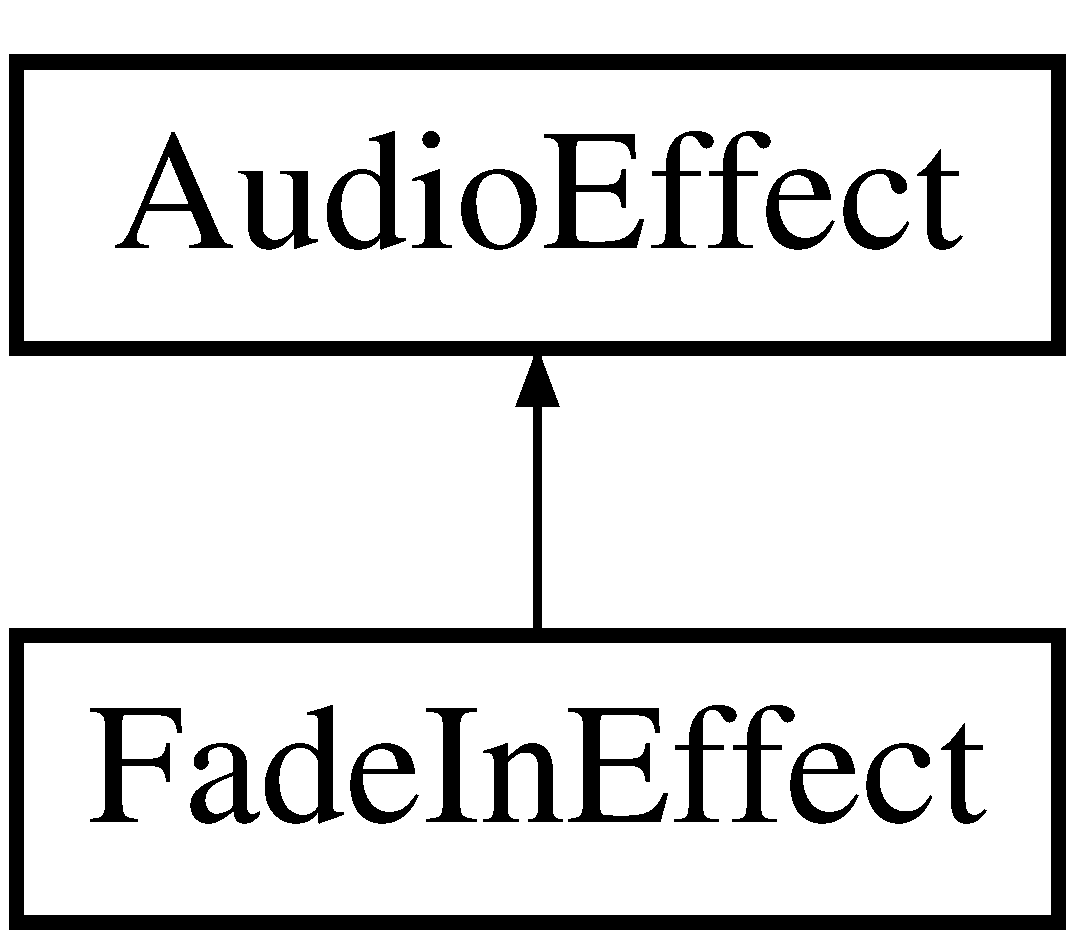
\includegraphics[height=2.000000cm]{class_fade_in_effect}
\end{center}
\end{figure}
\subsection*{Public Member Functions}
\begin{DoxyCompactItemize}
\item 
\mbox{\Hypertarget{class_fade_in_effect_a5899b6e349fbdfb0c4af9d44a20e47e5}\label{class_fade_in_effect_a5899b6e349fbdfb0c4af9d44a20e47e5}} 
{\bfseries Fade\+In\+Effect} (float time=1.\+0f)
\end{DoxyCompactItemize}
\subsection*{Additional Inherited Members}


\subsection{Detailed Description}
\hyperlink{class_audio}{Audio} effect that applies a fade out effect to audio. 

The documentation for this class was generated from the following files\+:\begin{DoxyCompactItemize}
\item 
C\+:/\+Users/wsheng/\+Documents/\+Neumont/\+Q9/capstone/repo/project/\+Dynamic\+Music/Fade\+In\+Effect.\+h\item 
C\+:/\+Users/wsheng/\+Documents/\+Neumont/\+Q9/capstone/repo/project/\+Dynamic\+Music/Fade\+In\+Effect.\+cpp\end{DoxyCompactItemize}

%--- End generated contents ---

% Index
\backmatter
\newpage
\phantomsection
\clearemptydoublepage
\addcontentsline{toc}{chapter}{Index}
\printindex

\end{document}
